%%%%%%%%%%%%%%%%%%%%%%%%%%%%%%%%%%%%%%%%%
% Stylish Curriculum Vitae
% LaTeX Template
% Version 1.1 (September 10, 2021)
%
% This template originates from:
% https://www.LaTeXTemplates.com
%
% Authors:
% Stefano (https://www.kindoblue.nl)
% Vel (vel@LaTeXTemplates.com)
%
% License:
% CC BY-NC-SA 4.0 (https://creativecommons.org/licenses/by-nc-sa/4.0/)
%
%%%%%%%%%%%%%%%%%%%%%%%%%%%%%%%%%%%%%%%%%
% !TEX program = xelatex
\documentclass[a4paper, oneside, final, 12pt]{scrartcl} % Paper options using the scrartcl class

\usepackage{fontspec} % for other font
\usepackage{xeCJK} % for chinese font
\usepackage{hyperref} % for hyper web link
\usepackage{multirow} % for tabular table in learning progress
\usepackage{graphicx} % for image insersion
\usepackage[export]{adjustbox} % for image frame
\usepackage{setspace}
\usepackage{array}
% Define typographic struts, as suggested by Claudio Beccari
%   in an article in TeX and TUG News, Vol. 2, 1993.
\usepackage{mathptmx}
\usepackage{scrlayer-scrpage} % Provides headers and footers configuration
\usepackage{titlesec} % Allows creating custom \section's
\usepackage{marvosym} % Allows the use of symbols
\usepackage{tabularx,colortbl} % Advanced table configurations
% \usepackage{ebgaramond} % Use the EB Garamond font
\usepackage{microtype} % To enable letterspacing
\usepackage{pdfpages} % for showing pdf
\usepackage{pdflscape}
\usepackage{enumitem}
\usepackage{subcaption}
\usepackage{listings}   % highlight the python code
\usepackage{xcolor}
\usepackage{multirow}
\usepackage{cite} %Imports biblatex package
\usepackage[ruled,linesnumbered]{algorithm2e}
\newcommand\mycommfont[1]{\normalsize\ttfamily\textcolor{blue}{#1}}
\SetCommentSty{mycommfont}
% \usepackage[backend=bibtex,bibencoding=ascii,style=authoryear,sorting=none]{bibtex}
% \addbibresource{reference.bib}
% setup the margin
\usepackage[top=1cm, bottom=1cm, right=2cm, left=2cm]{geometry}

% set the style of listing code
\definecolor{codegreen}{rgb}{0,0.6,0}
\definecolor{codegray}{rgb}{0.5,0.5,0.5}
\definecolor{codepurple}{rgb}{0.58,0,0.82}
\definecolor{backcolour}{rgb}{0.95,0.95,0.92}

\lstdefinestyle{mystyle}{
    backgroundcolor=\color{backcolour},   
    commentstyle=\color{codegreen},
    keywordstyle=\color{magenta},
    numberstyle=\tiny\color{codegray},
    stringstyle=\color{codepurple},
    basicstyle=\ttfamily\footnotesize,
    breakatwhitespace=true,         
    breaklines=true,                 
    captionpos=b,                    
    keepspaces=true,                 
    numbers=left,                    
    numbersep=5pt,                  
    showspaces=false,                
    showstringspaces=false,
    showtabs=false,                  
    tabsize=2
}

\lstset{style=mystyle}

% set chinese and english font
\setmainfont{Times New Roman}
\setCJKmainfont[AutoFakeBold=true, AutoFakeSlant=true]{標楷體}

\titleformat{\section}{\Large\raggedright\bfseries}{}{0em}{}[\titlerule] % Section formatting
\titleformat{\subsection}{\large\raggedright\bfseries}{}{0em}{}
\titleformat{\subsubsection}{\normalsize\raggedright\bfseries}{}{0em}{}

% \pagestyle{scrheadings} % Print the headers and footers on all pages

% enable bold and slant chinese font
% \xeCJKsetup{AutoFakeBold=true, AutoFakeSlant=true}

% set the space at the front of paragraph
\setlength{\parindent}{2em}

% disable page number
\pagenumbering{gobble}

\newcommand{\gray}{\rowcolor[gray]{.90}} % Custom highlighting for the work experience and education sections
\newcommand{\Tstrut}{\rule{0pt}{2.6ex}}         % = `top' strut
\newcommand{\Bstrut}{\rule[-0.9ex]{0pt}{0pt}}   % = `bottom' strut
\newcommand{\Tstruth}{\rule{0pt}{4ex}}         % = `top' strut for header
\newcommand{\Bstruth}{\rule[-2.5ex]{0pt}{0pt}}   % = `bottom' strut for header

%----------------------------------------------------------------------------------------
%	FOOTER SECTION
%----------------------------------------------------------------------------------------

% \renewcommand{\headfont}{\normalfont\rmfamily\scshape} % Font settings for footer

% \cofoot{
% \fontsize{12.5}{17}\selectfont % Letter spacing and font size

% \textls[150]{123 Broadway {\large\textperiodcentered} City {\large\textperiodcentered} Country 12345}\\ % Your mailing address
% {\Large\Letter} \textls[150]{john@smith.com \ {\Large\Telefon} (000) 111-1111} % Your email address and phone number
% }

%----------------------------------------------------------------------------------------
\begin{document}

%----------------------------------------------------------------------------------------
%	HEADER SECTION
%----------------------------------------------------------------------------------------


\begin{center}
    {\fontsize{18}{30}\textbf{Data Mining Assignment 2 \\ Classification}}
\end{center}

\begin{center}
  Bo-Han Chen (陳柏翰) \\
  Student ID:312551074 \\
  bhchen312551074.cs12@nycu.edu.tw
\end{center}

\section{Experiment Environment \& Usage}

\begingroup
\raggedright

\subsection{Environment}

\begin{itemize}
  \item OS: Windows 10 22H2
  \item Hardware: Intel(R) Xeon(R) CPU E3-1231 v3 @ 3.40GHz
  \item Python 3.12.0
\end{itemize}

\section{Data Preprocessing}

\subsection{Data Overview}

The given dataset contains 44939 patients' information, including 81 features and 1 label representing whether the patient has died.
Among the 81 features, 23 features are categorical and the rest are numerical.

\subsubsection{Categorical Features}

Categorical features contain two types of data, including \emph{bool} and \emph{object}.
After visualizing the data, I found several features that are highly related to the result of death.
The details are shown as follows:

\begin{figure}[ht]
  \centering
  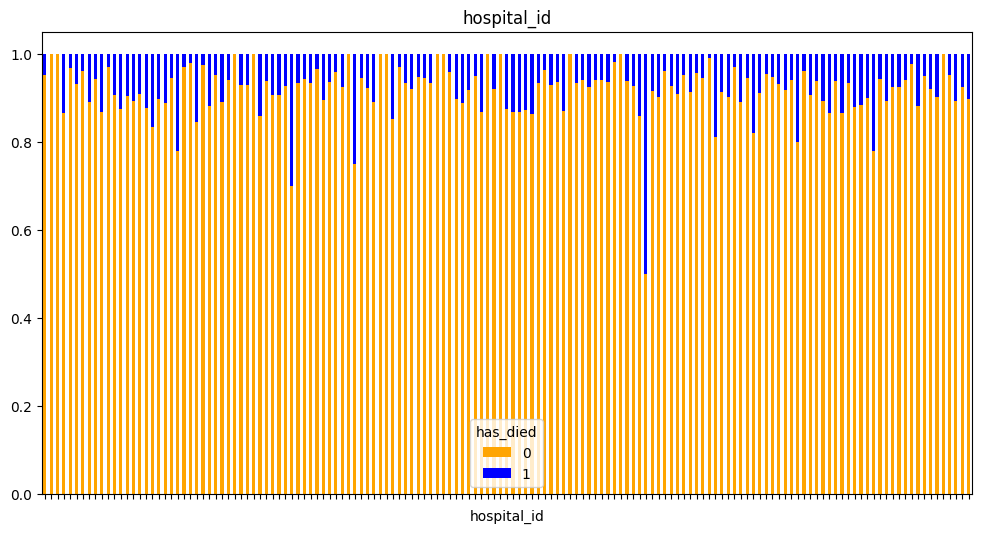
\includegraphics[width=0.9\textwidth]{"./image/dataset/hospital_id_dis.png"}
  \caption{Percentage of Death in Different Hospital}
  \label{fig:hospital}
\end{figure}

\begin{figure}[ht]
  \centering
  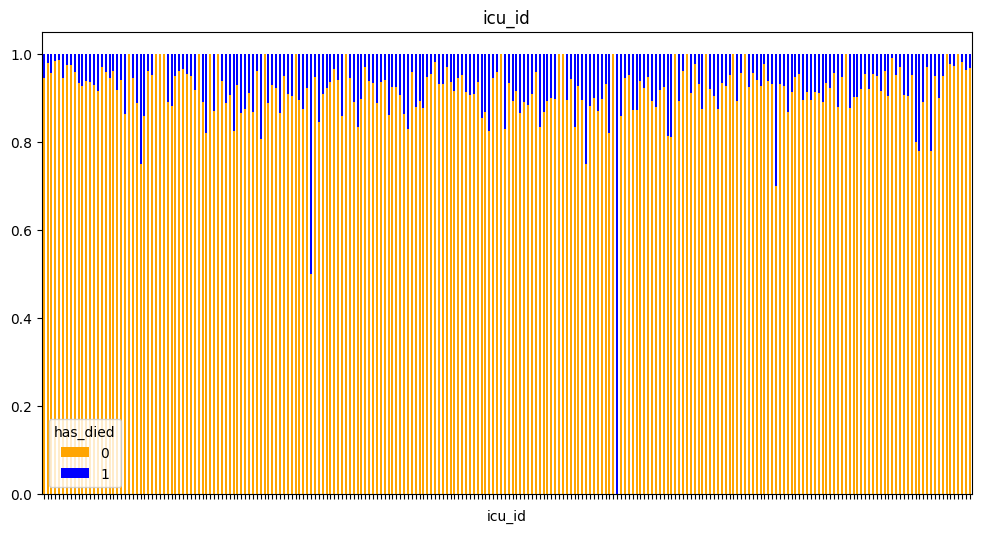
\includegraphics[width=0.9\textwidth]{"./image/dataset/icu_id_dis.png"}
  \caption{Percentage of Death in Different ICU}
  \label{fig:icu}
\end{figure}

From the figure \ref{fig:hospital} and figure \ref{fig:icu}, 
we can see that some of the hostipal and icu are has higher death rate than others.
So it's reasonable to assume that the hostipal and icu information are related to the result of death in this dataset,
and it is necessary to keep these features. \\

Since there are some missing values in the categorical features, 
so we can first analyze the relationship between missing values and result of death,
and then decide the way to transform the missing values.
First, I analyze the percentage of missing values in each feature in figure \ref{fig:missing_cat}.
From the figure, we can see that the missing values accounts for proportion of 0.75\% to 1.75\%
in most of the categorical features, now we can look into the 
features with high percentage of missing values.

\begin{figure}[ht]
  \centering
  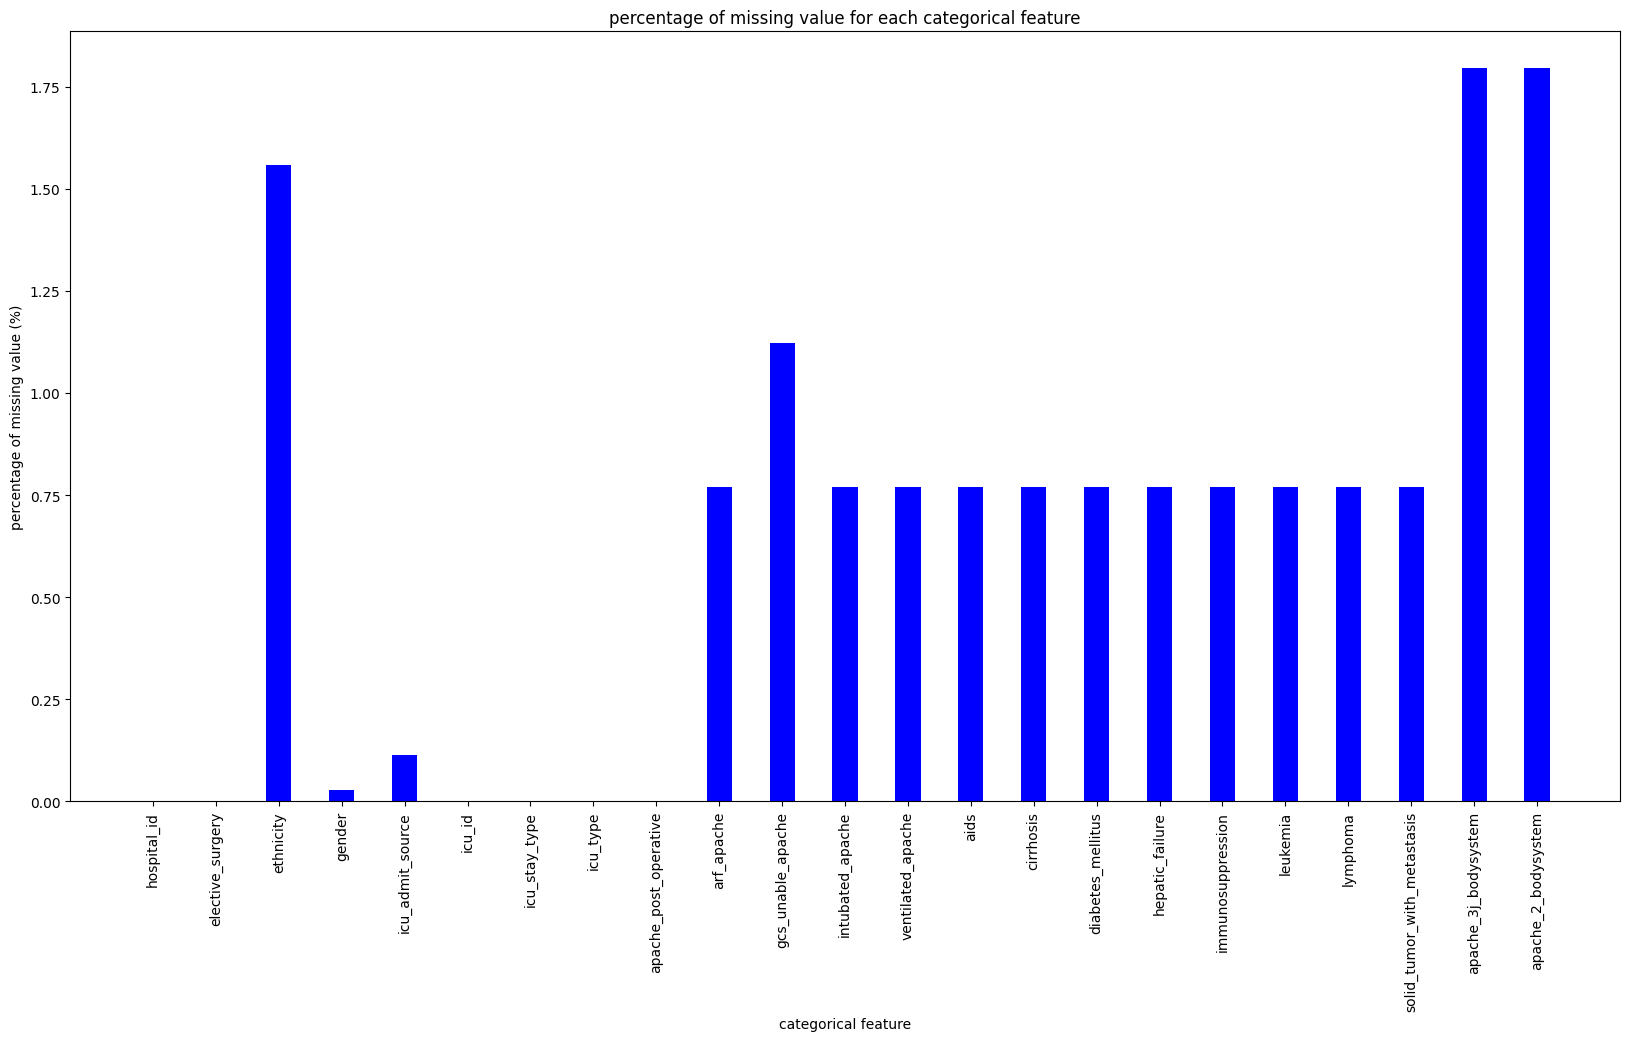
\includegraphics[width=0.9\textwidth]{"./image/dataset/cat_nan_percentage.png"}
  \caption{Percentage of Missing Values in Categorical Features}
  \label{fig:missing_cat}
\end{figure}

For feature \emph{apache\_2\_bodysystem} and \emph{apache\_3j\_bodysystem} and \emph{ethnicity},
the relationship between missing values and death rate is shown in 
figure \ref{fig:apache_2}, figure \ref{fig:apache_3j} and figure \ref{fig:ethnicity}
From the figure, we can see that the missing values 
in these three features still contains some information about the result of death,
so it's not reasonable to simply drop these missing values.
For the rest of categorical features that also contains missing values,
the missing values are also accounts for a small proportion of death rate.
Although these related death result represents a very small proportion of the whole dataset,
it's still necessary to keep these missing values to avoid losing important information.

\newpage


\begin{figure}[ht]
  \centering
  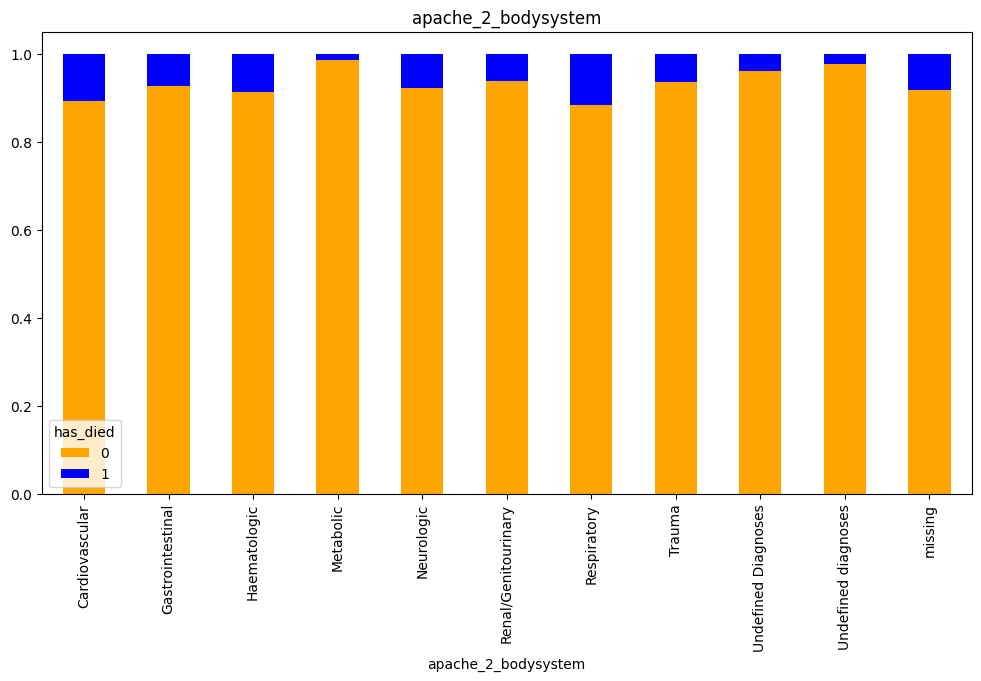
\includegraphics[width=0.62\textwidth]{"./image/dataset/apache_2_dis.png"}
  \caption{Percentage of Death in Different apache\_2\_bodysystem}
  \label{fig:apache_2}
\end{figure}

\begin{figure}[ht]
  \centering
  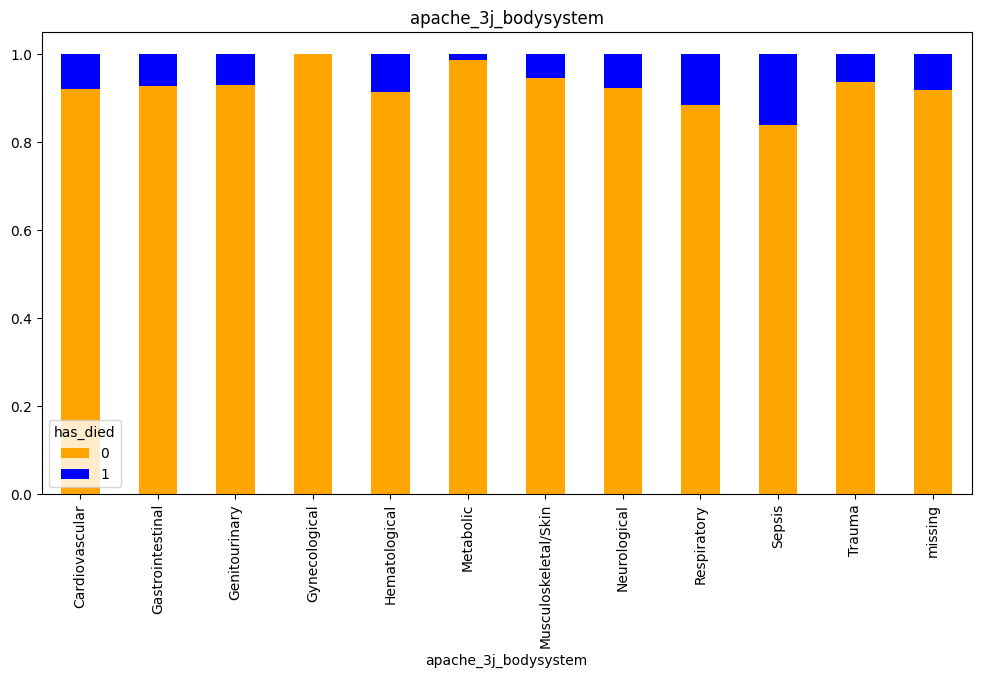
\includegraphics[width=0.62\textwidth]{"./image/dataset/apache_3j_dis.png"}
  \caption{Percentage of Death in Different apache\_3j\_bodysystem}
  \label{fig:apache_3j}
\end{figure}

\begin{figure*}[!b]
  \centering
  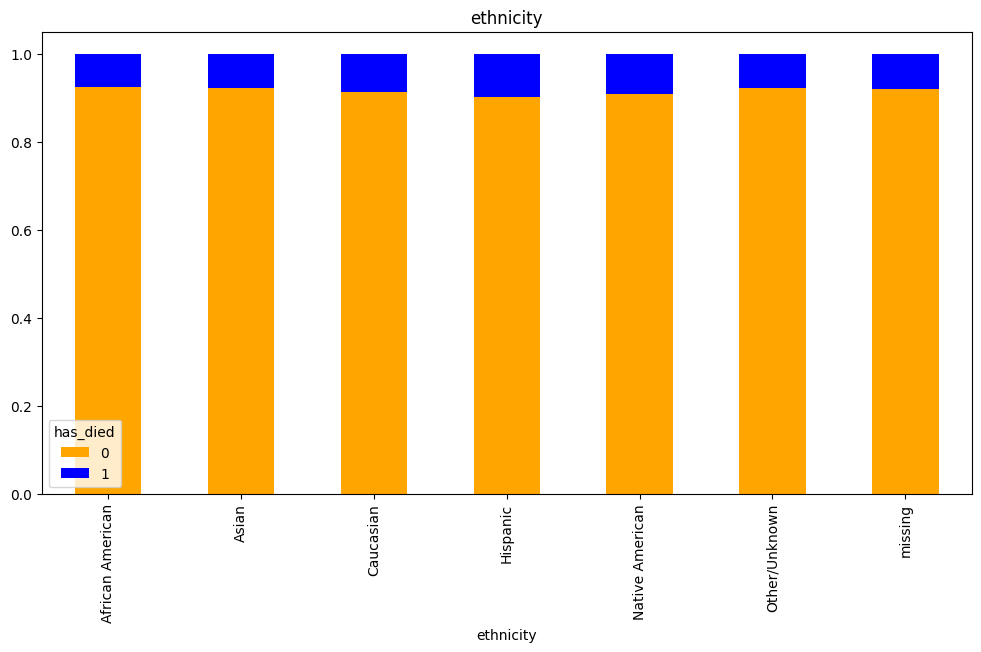
\includegraphics[width=0.62\textwidth]{"./image/dataset/ethnicity_dis.png"}
  \caption{Percentage of Death in Different ethnicity}
  \label{fig:ethnicity}
\end{figure*}

\newpage

\subsubsection{Numerical Features}

For numerical features, I first analyze the percentage of 
missing values in figure \ref{fig:num_nan_percentage}.
From the figure we can see the proportion of missing values in most of numerical features
is much higher than the categorical features.
For further analysis, I fill the missing values with the mean value of each feature,
which can minimize the impact of missing values.

\begin{figure}[h]
  \centering
  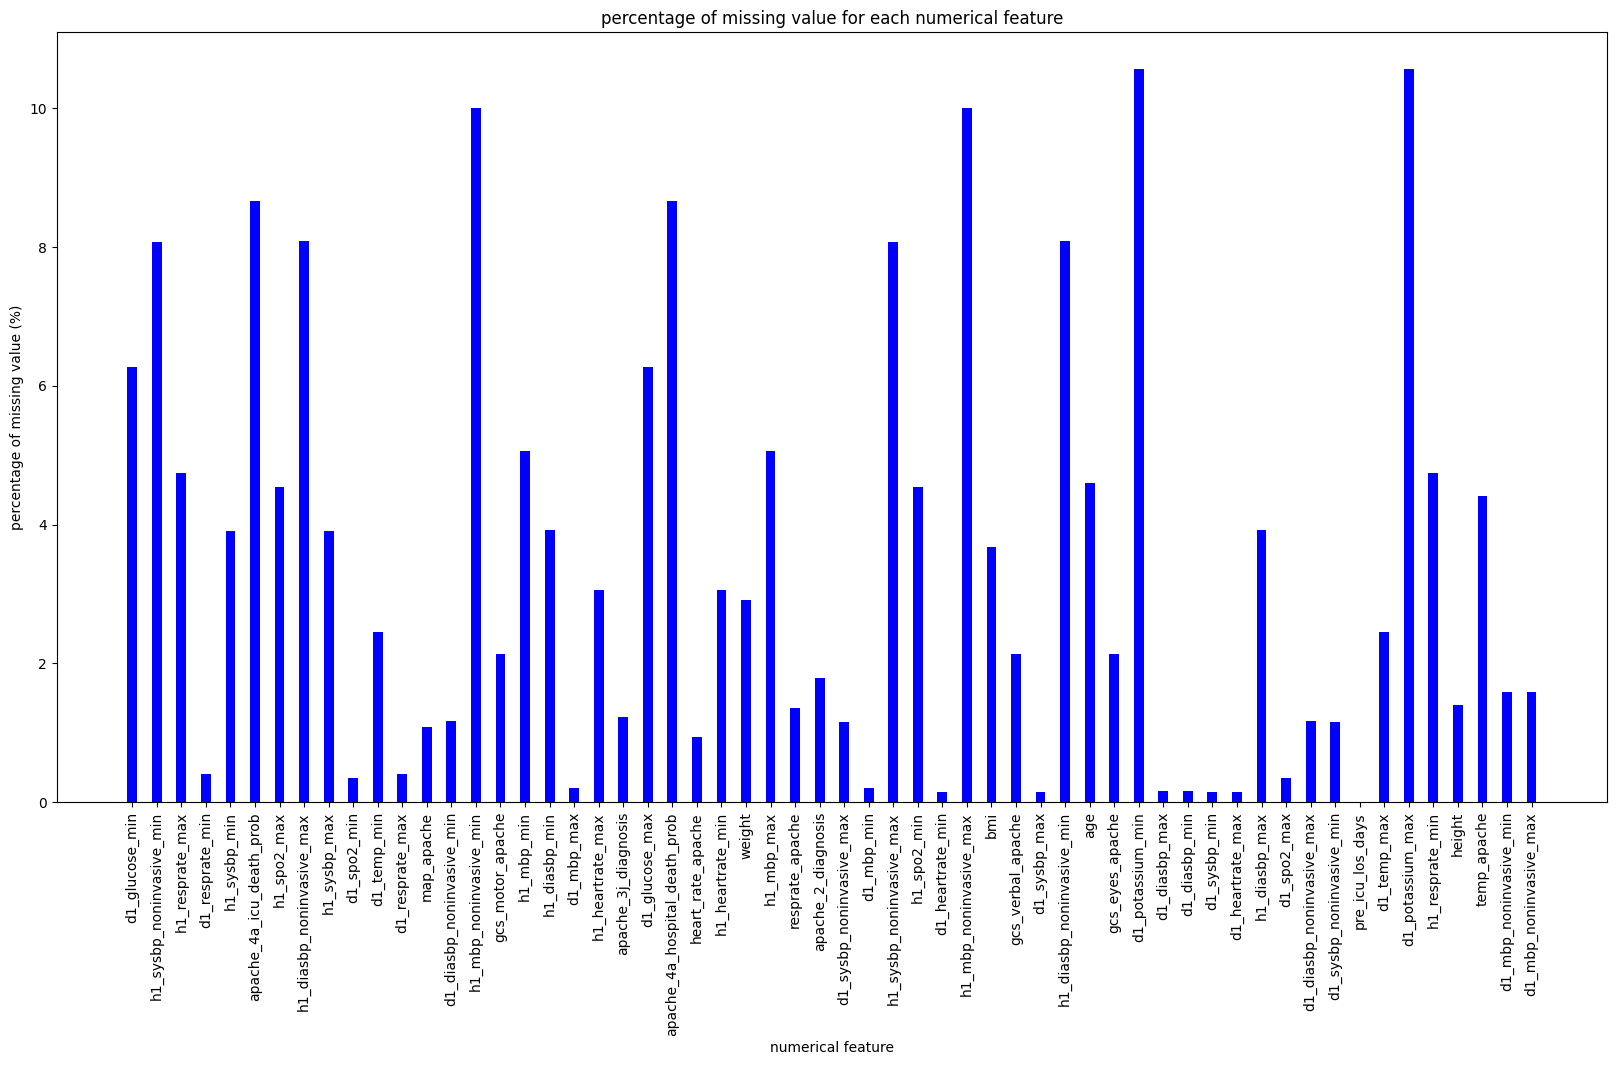
\includegraphics[width=0.9\textwidth]{"./image/dataset/num_nan_percentage.png"}
  \caption{Percentage of Missing Values in Numerical Features}
  \label{fig:num_nan_percentage}
\end{figure}

Figure \ref{fig:bmi} show the distribution of bmi in different result of death.
From the figure, we can see the trend of bmi value among our dataset,
and the percentage of death is quite similar in different bmi value.
An other interesting discovery is that there are some abnormal distribution near the bmi value 70,
which I think is the outlier of this dataset at the first glance.
However, after further analysis, I found that the same distribution trend can be found in
feature \emph{weight} from figure \ref{fig:weight},
which means the abnormal distribution may be casued by realistic reasons,
such as some diagnosis or treatment may cause the patient to gain weight.

\begin{figure}[h]
  \centering
  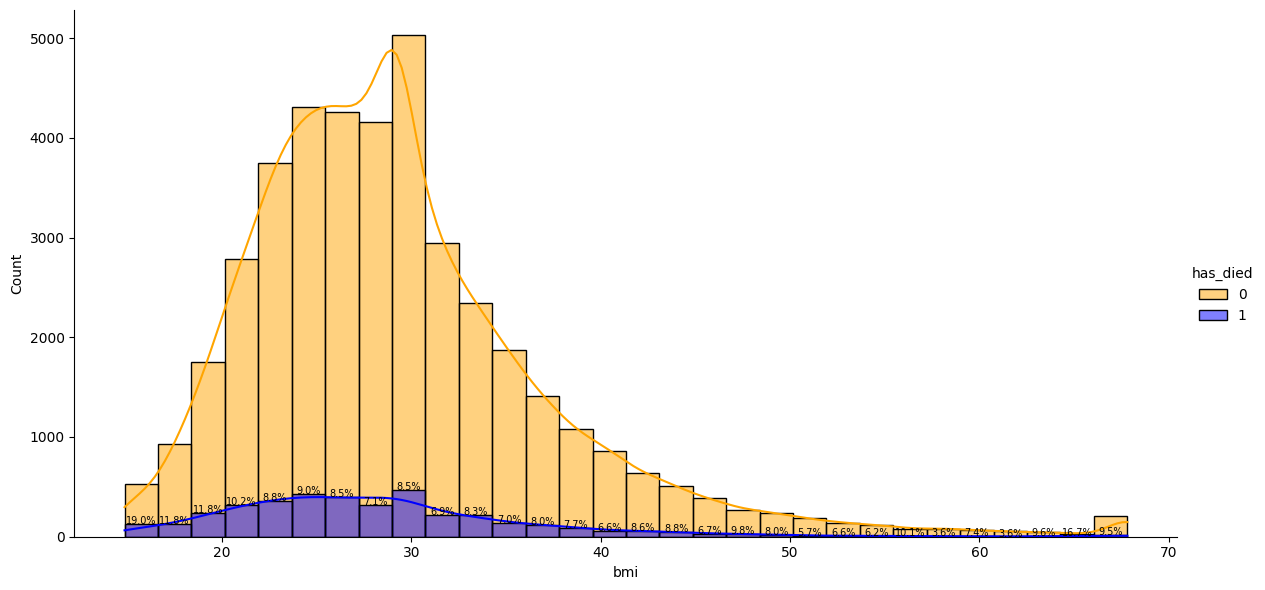
\includegraphics[width=0.9\textwidth]{"./image/dataset/bmi_dis.png"}
  \caption{Distribution of bmi}
  \label{fig:bmi}
\end{figure}

\begin{figure}[h]
  \centering
  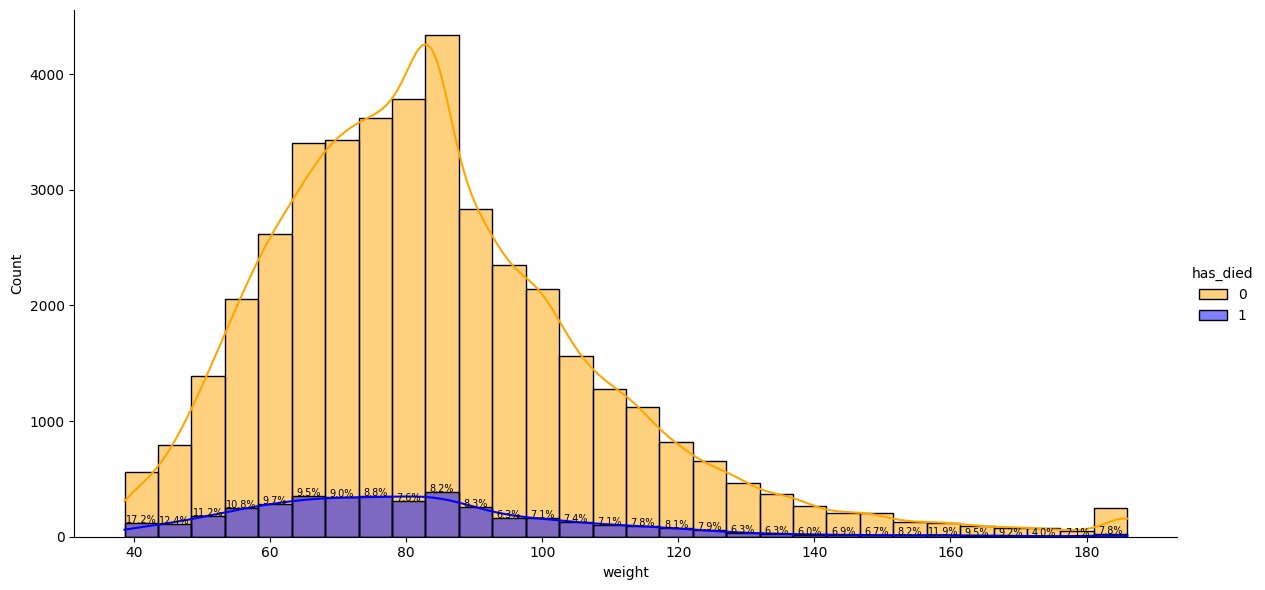
\includegraphics[width=0.9\textwidth]{"./image/dataset/weight_dis.png"}
  \caption{Distribution of weight}
  \label{fig:weight}
\end{figure}

The discovery about outliers can be found in 
feature \emph{apache\_4a\_hospital\_death\_prob} and \emph{apache\_4a\_icu\_death\_prob}.
From figure \ref{fig:apache_4a_hospital_death_prob} and figure \ref{fig:apache_4a_icu_death_prob},
we can see there are some negative values in these two features,
which is obviously the outliers when representing the probability of death.
To dealing with these outliers, I replace them with NaN values and use imputation for restoring,
expect this operation can let the new value be more realistic.
The details of imputation will be mentioned in the following section.

\begin{figure}[h]
  \centering
  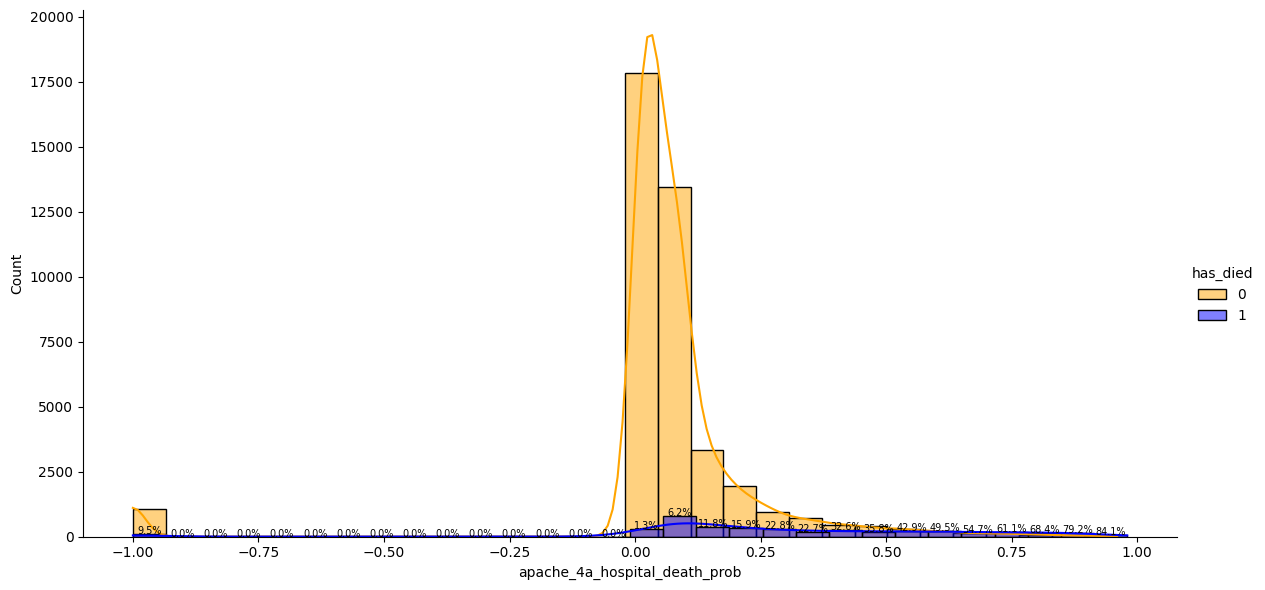
\includegraphics[width=0.9\textwidth]{"./image/dataset/hospital_death_prob_dis.png"}
  \caption{Distribution of apache\_4a\_hospital\_death\_prob}
  \label{fig:apache_4a_hospital_death_prob}
\end{figure}

\begin{figure}[h]
  \centering
  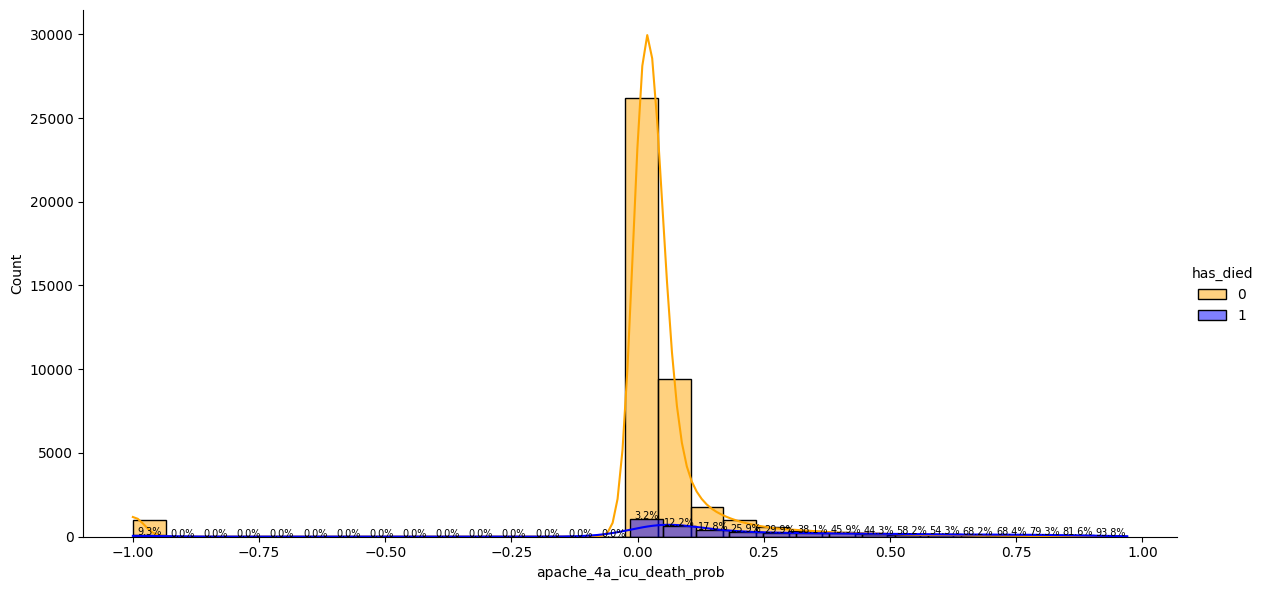
\includegraphics[width=0.9\textwidth]{"./image/dataset/icu_death_prob_dis.png"}
  \caption{Distribution of apache\_4a\_icu\_death\_prob}
  \label{fig:apache_4a_icu_death_prob}
\end{figure}

\subsection{Feature Encoding}

For this dataset, I tried several encoding method for categorical feature transformation,
since data transformation will also lead to different feature selected for training,
so we can 

% \newpage

% reftest\cite{zaki1997new}

\endgroup

% \bibliographystyle{unsrt} % We choose the "plain" reference style
% \bibliography{reference} % Entries are in the "references.bib" file

\end{document}